\chapter{Onde piane} 

\begin{figure}[h]
    \centering
    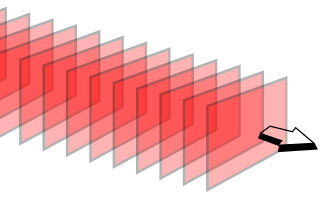
\includegraphics{Plane_wave_wavefronts_3D.png}
    
\end{figure} 

\newpage 

\section{Onde piane - Equazioni e coefficienti}
\footnote{FWC - pag 275 | 6.2 Uniform plane waves in a perfect dielectric} 

Ricordando le leggi di Maxwell, possiamo applicarle alle onde piane: 

{\Large \begin{equation}
    \begin{cases}
        \nabla \cdot \vec{E} = 0 \\ 
        \nabla \cdot \vec{H} = 0 \\ 
        \nabla \times \vec{E} = -\mu \frac{\partial \vec{H}}{\partial t} \\ 
        \nabla \times \vec{H} = \varepsilon \frac{\partial \vec{E}}{\partial t}
    \end{cases}
\end{equation}} 

In fisica matematica, un'onda piana è un'onda a frequenza costante i cui fronti d'onda sono infiniti piani paralleli perpendicolari alla direzione di propagazione, e la cui distanza picco-picco è costante. \\ 

L'onda piana rappresenta un'astrazione matematica che non corrisponde ad alcun fenomeno fisico equivalente in senso stretto, poiché a partire da una descrizione analitica esatta si ottiene un'onda che per essere generata necessita di una sorgente di lunghezza infinita. \\ \\
L'onda piana è tuttavia utilizzata per approssimare il caso in cui la sorgente dell'onda è posta a distanza infinita dal punto di osservazione del fronte d'onda considerato, che viene quindi assunto localmente piano. \\ \\ 
Una caratteristica che la differenzia da altri tipi di propagazione ondosa, come l'onda sferica (tridimensionale) o quella circolare (in due dimensioni), è l'assenza di attenuazione isotropica nello spazio, in virtù della direzionalità dell'emissione e della propagazione di energia associata all'onda. L'unica attenuazione che si verifica è dovuta all'eventuale assorbimento da parte del materiale del mezzo di propagazione attraversato. 

\footnote{Wikipedia - Onde piane} \\

Possiamo scrivere l'onda piana come un'onda che si propaga 
lungo l'asse z (asse scelto da noi come quello di propagazione, l'onda piana può propagarsi anche negli altri due assi) 
come: \\ 

{\Large \begin{equation}
    E_x (z, t) = f_1 (t-\frac{z}{v}) + f_2 (t-\frac{z}{v}) 
\end{equation}}

dove: 
{
    \Large
    \begin{equation}
        v = \frac{1}{\sqrt{\mu \varepsilon}} 
    \end{equation}
}

v è la velocità della luce nel mezzo. \\ \\ 

Possiamo scrivere: 

{\Large \begin{equation}
    E_x ^{+} = f_1 (t - \frac{z}{v})
\end{equation}}

l'onda che si propaga lungo l'asse z. 

{\Large \begin{equation}
    E_x ^{-} = f_2 (t + \frac{z}{v})
\end{equation}} 

l'onda che si propaga lungo l'asse -z. \\ \\ 


Con lo stesso principio, e sempre grazie alle leggi di Maxwell, possiamo scrivere: 

{\Large \begin{equation}
    \begin{split}
        H_y 
        &= H_y ^{+} H_y ^{-} 
        \\
        &= \frac{E_x ^{+}}{\eta} - \frac{E_x ^{-}}{\eta} 
    \end{split}
\end{equation}}

dove: \\ 

{\Large \begin{equation}
    \eta = \sqrt{\frac{\mu}{\varepsilon}}
\end{equation}}

$\eta$ si può ricavare anche come: 

{\Large \begin{equation}
    \eta = \frac{E_x}{H_y}    
\end{equation}} 

Grazie a questo rapporto, $\eta$ prende il nome di Impedenza intrinsica nel mezzo. 

Nel vuoto: 
{\Large \begin{equation}
    \eta_o = \sqrt{\frac{\mu_o}{\varepsilon_o}} = 376,73 [\Omega] \approx 120 \pi [\Omega]
\end{equation}}

\begin{tcolorbox}
$\Omega$ (lettera greca Omega, ma in questo caso rappresente l'unità di misura Ohm)  è la stessa 
unità di misura usata nei circuiti elettronici. 
    
\end{tcolorbox}

Quello che abbiamo visto con $E_x$ e $H_y$, è possibile anche con $E_y$ e $H_x$. 

{\Large \begin{equation}
    \begin{cases}
        E_y = f_3 (t-\frac{z}{v}) + f_4 (t+\frac{z}{v}) = E_y ^{+} + E_y ^{-} \\ \\
        H_x = - \frac{E_y ^{+}}{\eta} + \frac{E_y ^{-}}{\eta}     
    \end{cases}
\end{equation}} 

Quindi possiamo scrivere: 

{\Large \begin{equation}
    \begin{cases}
        \frac{E_x ^{+}}{H_y ^{+}} = -\frac{E_y ^{+}}{H_x ^{+}} = \eta \\ 
        \frac{E_x ^{-}}{H_y ^{-}} = -\frac{E_y ^{-}}{H_x ^{-}} = - \eta
    \end{cases}
\end{equation}} 

Da queste relazioni possiamo scrivere, se E è perpenicolare a H: 

{\Large \begin{equation}
    E = \eta H
\end{equation}} 




Dal Teorema di Poynting, possiamo scrivere la potenza dell'onda lungo l'asse z come: 

{\Large \begin{equation}
    \begin{split}
        P_z ^{+} 
        &= E_x ^{+} H_y ^{+} - E_y ^{+} H_x ^{+} 
        \\
        &= \frac{1}{\eta} (E_x ^{+^{2}} + E_y ^{+^{2}}) 
    \end{split}
\end{equation}}

\begin{figure}[h]
    \centering
    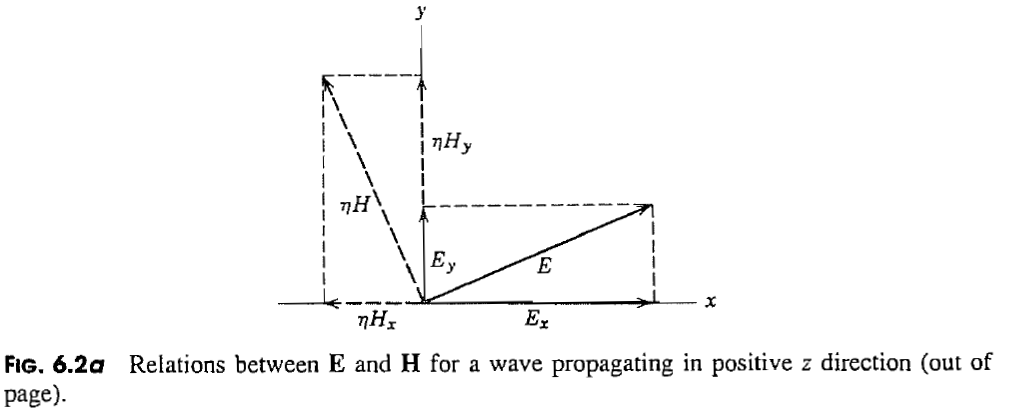
\includegraphics[scale = 0.6]{E and H in a plane wave.PNG}
\end{figure} 

\footnote{FWC - pag 277} 

\newpage 

\section{Onde piane in forma fasoriale} 

\footnote{FWC - pag 275 | 6.2 Uniform plane waves in a perfect dielectric} 

Estendendo l'analisi in forma fasoriale: 

{\Large \begin{equation}
    \begin{cases}
        E_x (z) = E_1 e^{-\jmath \kappa z} + E_2 e^{\jmath \kappa z} \\ 
        \eta H_y (z) = E_1 e^{-\jmath \kappa z} - E_2 e^{\jmath \kappa z} \\ \\ 

        E_y (z) = E_3 e^{-\jmath \kappa z} + E_4 e^{\jmath \kappa z} \\ 
        \eta H_x (z) = - E_3 e^{-\jmath \kappa z} + E_4 e^{\jmath \kappa z}

    \end{cases}
\end{equation}} 


dove: 

{\Large \begin{equation}
    \kappa = \frac{\omega}{v} = v \sqrt{\mu \varepsilon}
\end{equation}}

$\kappa$ è chiamata numero d'onda (in inglese wave number). \\ 
$\kappa$ è la fase dell'onda, in cui nelle onde piane è costante. \\ 

La lunghezza dell'onda $\lambda$ (si legge lambda) è il valore di z in cui la fase cambia di $2 \pi$. 

{\Large \begin{equation}
    \kappa \lambda = 2 \pi 
    \Rightarrow \kappa = \frac{2 \pi}{\lambda}
\end{equation}} 


{\Large \begin{equation}
    \lambda = \frac{2 \pi}{\kappa} = \frac{2 \pi}{\omega \sqrt{\mu \varepsilon}} = \frac{v}{f} 
\end{equation}}

Per calcolare la lunghezza d'onda nel vuoto, possiamo sostituire a v la velocità della luce, indicata anche come c. \\ 

In ottica, si sceglie di indicare $\lambda$ come n, dove n prende il nome di indice refrattivo (in inglese refractive index). 

{\Large \begin{equation}
    n = \frac{c}{v} = \sqrt{\frac{\mu \varepsilon}{\mu_o \varepsilon_o}}
\end{equation}}

Per molti materiali in ottica, e anche per materiali non magnetici, $\mu = \mu_o$

\newpage

\section{Polarizzazione delle onde piane} 
\footnote{FWC - pag 280 | 6.3 Polarization of plane waves} 

Se diverse onde piane hanno la stessa direzione di propagazione, 
possiamo sovrapporre queste onde per un mezzo lineare. \\ 

L'orientazione dei campi vettoriali, sia della singola onda che delle altre, è descritta dalla polarizzazione delle onde 
(in questo inserto parleremo solo di onde della stessa frequenza). \\ 

Prendiamo solo un'onda lungo l'asse z, usando la rappresentazione fasoriale e assumiamo sia x e y componenti del campo elettrico. \\ \\ 
L'espressione generale per quest'onda è la seguente: 

{\Large \begin{equation}
    \vec{E} = (\hat{x} E_1 + \hat{y} E_2 e^{\jmath \psi } e^{-\jmath \kappa z})
\end{equation}}

dove $E_1$ e $E_2$ sono reali e $\psi$ (si legge psi) è l'angolo tra le componenti x e y. \\ 

Il corrispondente campo magnetico è: 

{\Large \begin{equation}
    \vec{H} = \frac{1}{\eta} (-\hat{x} E_2 e^{\jmath \psi} + \hat{y}E_1) e^{-\jmath \kappa z}
\end{equation}}

Le onde possono essere anche non polarizzate. \\ 

Ci sono diverse classi di polarizzazione che dipendono dalla fase e dalle ampiezze di $E_1$ e $E_2$. \\ \\ 

\newpage 

\subsection{Polarizzazione lineare o planare}

\begin{figure}[h]
    \centering
    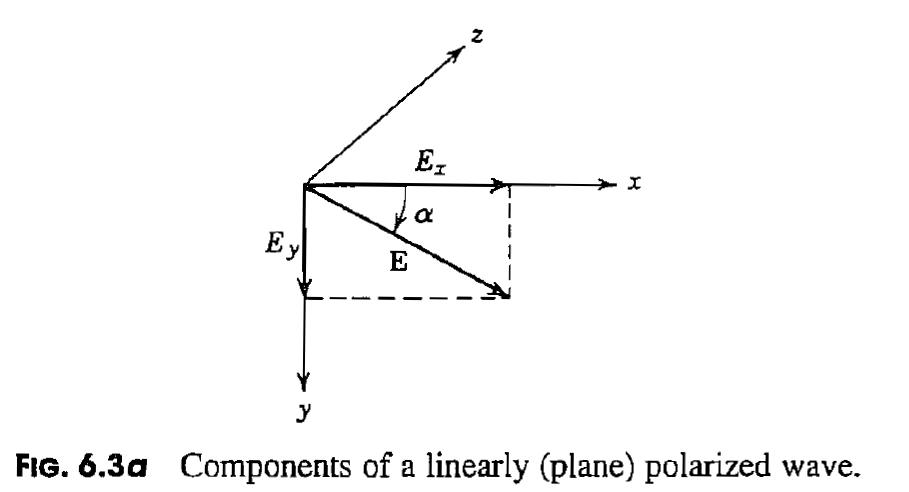
\includegraphics[scale = 0.8]{Linearly polarized wave.PNG}
    
\end{figure}

\footnote{FWC - pag 280}

Se i due campi sono in fase, cioè $\psi = 0$, ogni piano in z sarà definito da un angolo rispetto all'asse x chiamato $\alpha$ (si legge alfa) come: 

{\Large \begin{equation}
    \alpha = \arctan \frac{E_y}{E_x} = \arctan \frac{E_2}{E_1}
\end{equation}}

\begin{tcolorbox}
    $\arctan$ è l'inverso della funzione tangente. \\ $\arctan$ = $\tan ^{-1}$ 
\end{tcolorbox}

Questo angolo è reale, quindi è lo stesso per tutti i valori di z e t. \\ 

Siccome $\vec{E}$ mantiene la sua direzione nello spazio, questa polarizzazione è chiamata lineare, o polarizzazione planare perchè il vettore 
del campo elettrico definisce un piano che si propaga lungo la direzione z. \\ 

\newpage 

\subsection{Polarizzazione circolare} 

\begin{figure}[h]
    \centering
    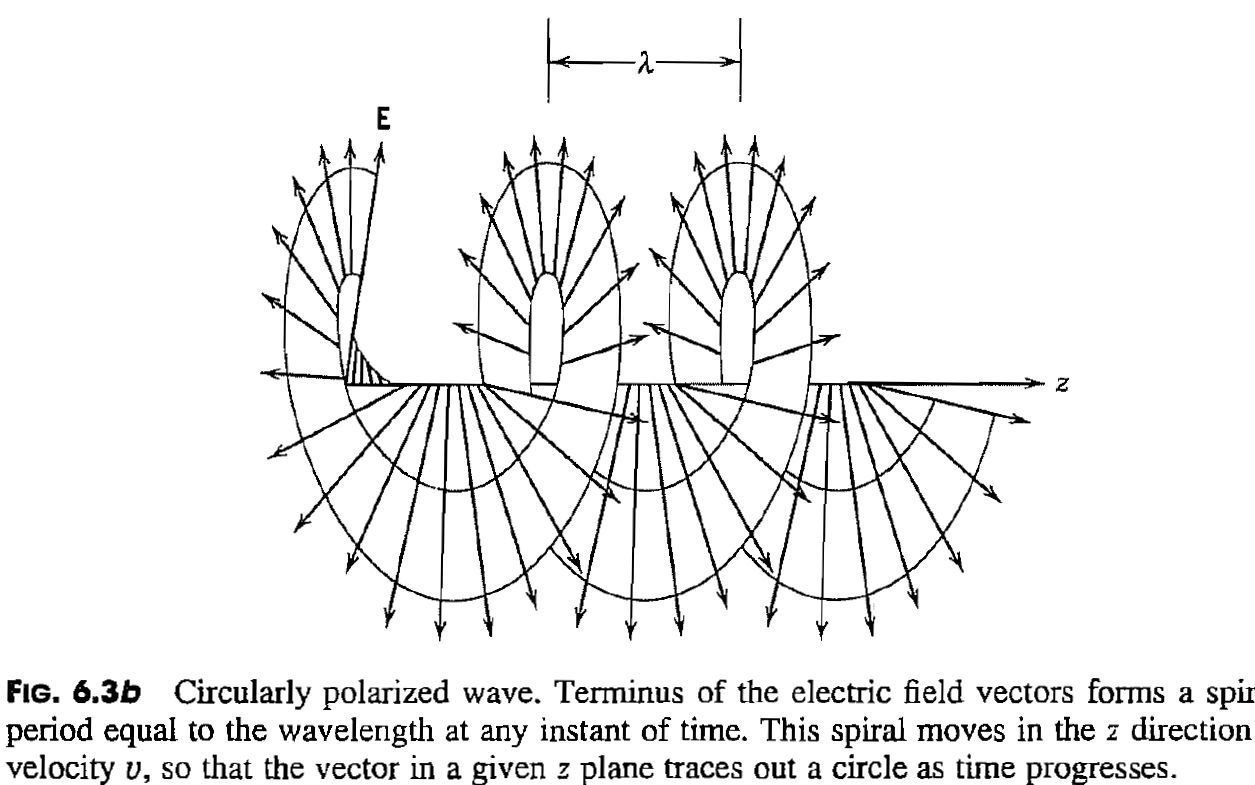
\includegraphics[scale = 0.5]{Circularly polarized wave.PNG}
    
\end{figure}

\footnote{FWC - pag 281}

Nella polarizzazione circolare: 

{\Large \begin{equation}
    \begin{cases}
        E_1 = E_2 \\ 
        \psi = \pm  \frac{\pi}{2}   
    \end{cases}
\end{equation}}

Quindi, con le dovute sostituzioni: 

{\Large \begin{equation}
    \begin{split}
    \vec{E} 
    &= (\hat{x} E_1 + \hat{y} E_2 e^{\jmath \psi } e^{-\jmath \kappa z}) 
    \\
    &\Rightarrow  \vec{E} = (\hat{x} + \pm \jmath \hat{y}) E_1 e^{- \jmath \kappa z}
    \end{split}
\end{equation}}

L'ampiezza di $\vec{E}$ è $\sqrt{2} E_1$ e il vettore $\vec{E}$ è un vettore che si muove in modo circolare. \\ 

La forma instantanea di un'onda polarizzata circolarmente: 

{\Large \begin{equation}
    \begin{split}
        \vec{E} (z, t) &= \Re [(\hat{x} + \pm \jmath \hat{y}) E_1 e^{- \jmath \kappa z} ]  \\
        &= E_1 [\hat{x} \cos(\omega t - \kappa z) \mp \hat{y} \sin(\omega t -\kappa z) ]    
    \end{split}
\end{equation}}

La somma del quadrato delle forme instantanee di $E_x$ e $E_y$ da: 

{\Large \begin{equation}
    \begin{split}
        E_x ^{2} (z, t) + E_y ^{2} (z, t) 
        &= E_1 ^{2} [\cos^{2}(\omega t - \kappa z) + \sin^{2}(\omega t - \kappa z)] 
        \\
        &= E_1 ^{2}
    \end{split}
\end{equation}}

Equazione che definisce un cerchio. \\ 

L'angolo instantaneo $\alpha$ rispetto all'asse x è: 

{\Large \begin{equation}
    \begin{split}
        \alpha 
        &= \arctan \frac{E_y(z, t)}{E_x(z, t)} 
        \\
        &= \arctan (\frac{\sin(\omega t - \kappa z)}{\cos(\omega t - \kappa z)}) 
        \\
        &= \mp (\omega t - \kappa z)
    \end{split}
\end{equation}}


Dato un piano z, il vettore ruota con una velocità costante angolare di $\alpha = \mp \omega t$. \\ 

La propagazione dell'onda è di tipo epicicloidale (come il movimento di un cavatappi) lungo la direzione z con una velocità v. \\ 

Da notare che (per z = 0)
{\Large \begin{equation}
    \begin{cases}
     \psi = + \frac{\pi}{2} \Rightarrow \alpha = -\omega t \\ 
     \psi = - \frac{\pi}{2} \Rightarrow \alpha = \omega t 
    \end{cases}
\end{equation}}

Nel primo caso, l'onda si muove in senso anti-orario, nel secondo caso in senso orario. \\ 

Ricordando che se $E_1 = E_2$ e $\psi = \pm \frac{\pi}{2}$, il relativo campo magnetico di un'onda polarizzata in modo circolare è: 

{\Large \begin{equation}
    \vec{H} = \frac{E_1}{\eta} (\mp \jmath \hat{x} + \hat{y}) e^{- \jmath \kappa z}
\end{equation}}


\newpage 

\subsection{Polarizzazione elittica} 


\begin{figure}[h]
    \centering
    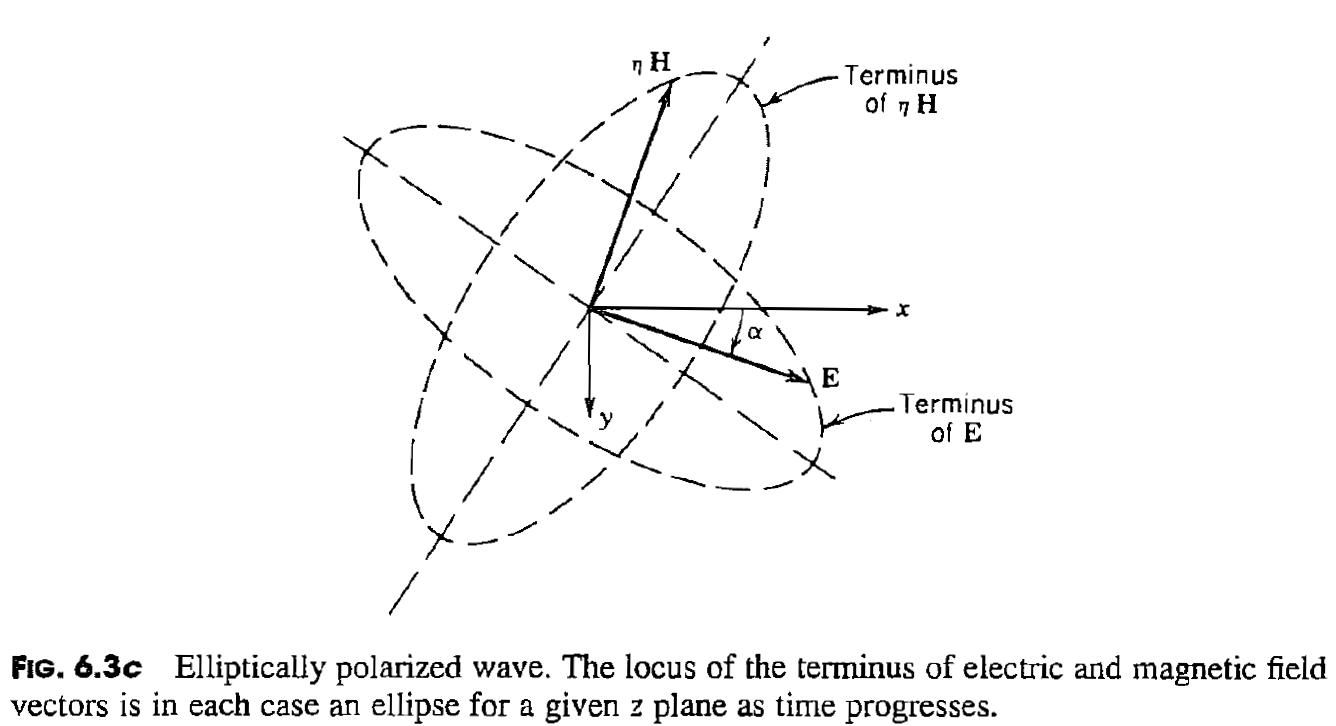
\includegraphics[scale = 0.5]{Elliptically polarized wave.PNG}
    
\end{figure}

\footnote{FWC - pag 282}


Per il caso generale, con $E_1 \neq E_2$ o $E_1 = E_2$, ma $\psi$ è diverso da 0 o da $\mp \frac{\pi}{2}$ . \\ \\
Quindi, per il caso generale, l'onda descrive una traiettoria di un elisse, quindi il nome di questa polarizzazione è detta elittica. \\ 

La forma instantanea di questo tipo d'onda è: 

{\Large \begin{equation}
    \begin{split}
        \vec{E} (z, t) &= \Re[(\hat{x} E_1 + \hat{y} E_2 e^{\jmath \psi}) e^{\jmath \omega t} e^{-\jmath \kappa z}] 
        \\ &= 
    \hat{x} E_1 \cos(\omega t - \kappa z) + \hat{y} E_2 \cos(\omega t - \kappa z + \psi) 
    \end{split}
\end{equation}}


Per un qualsiasi piano, poniamo z=0, 

{\Large \begin{equation}
    \begin{cases}
        E_x (z, t) = E_1 \cos(\omega t) \\ 
        E_y (z, t) = E_2 \cos(\omega t + \psi)     
    \end{cases}
\end{equation}}

